%\documentclass[a4paper,10pt]{article}
\documentclass[10pt]{scrartcl}
%\usepackage[IL2]{fontenc}
\usepackage[utf8x]{inputenc}
\usepackage[czech]{babel}
\usepackage{listings}  
\usepackage{amsfonts,amsmath,amssymb,graphicx,color}
%\usepackage[total={17cm,27cm}, top=2cm, left=2cm, includefoot]{geometry}
%\usepackage{fancyhdr}
\usepackage{fkssugar}
\usepackage{hyperref}
\usepackage{mhchem}

%\usepackage{caption}

%  Umožňuje rozdělovat obsah na více sloupců
\usepackage{multicol}
\usepackage{booktabs}
\usepackage{pgffor}


% FJFI Types of popi
\renewcommand{\popi}[2]{$\frac{#1}{[\jd{#2}]}$}

\renewcommand{\figurename}{Obr.}
\addto\captionsczech{\renewcommand{\figurename}{Obr.}}
\addto\captionsczech{\renewcommand{\tablename}{Tab.}}
\def\mean#1{\left< #1 \right>}


\newcommand{\MakeFJFIHead}{
\setlength{\parindent}{0cm}
\begin{multicols}{2}
\textsf{\textbf{\FJFISubject \hspace{6.25cm} \FJFIInstitute}\\
\textbf{\large{\FJFITitle}}}

\begin{tabular}{rlrl}
	 \textsf{Jméno:} & \textbf{\textsf\FJFIAuthor}    &      \textsf{Kolega:} & \textsf{\FJFICoauthor} \\[1.5pt]
	  \textsf{Kruh:} & \textbf{\textsf\FJFIGroup}     & \textsf{Číslo skup.:} & \textsf{\FJFICircle}   \\[1.5pt]
	\textsf{Měřeno:} & \textbf{\textsf{\FJFILabdate}} &  \textsf{Zpracování}: & \textsf{\FJFIWorktime}
\end{tabular}

\begin{flushright}


\includegraphics[scale=0.2]{../img/fjfi.pdf}
%\hspace{0.4cm}
%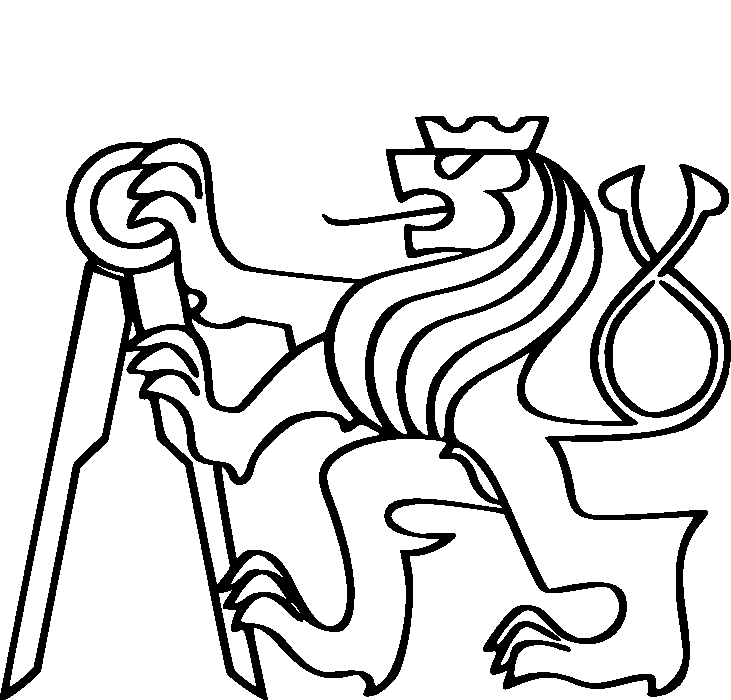
\includegraphics[scale=0.2]{../img/cvut.pdf}


\textsf{Klasifikace:} \hspace{3.2cm} 

\end{flushright}
\end{multicols}

\hrule
}




%  Nastaví autora, název, datum, skupinu měření apod. 
\newcommand{\FJFIInstitute}{FJFI~ČVUT~v~Praze}
%\newcommand{\Subject}{Základy fyzikálních měření}
\newcommand{\FJFISubject}{Fyzikální praktikum I}  %odkomentujte dle potřeby

%  Máte-li více spoluměřících než jednoho, vložte jen jejich příjmení
\newcommand{\FJFIAuthor}{Michal Červeňák}
\newcommand{\FJFICoauthor}{} 
\newcommand{\FJFIGroup}{Útorok} %den, kdy chodíte na praktika, nikoli obor
\newcommand{\FJFICircle}{1} %číslo skupiny v rámci praktika, nikoli kruh

%  Tato část bude v každém protokolu jiná, nezapomeňte upravit!
\newcommand{\FJFITitle}{4. Cavendishův experiment}
\newcommand{\FJFILabdate}{9.10.2017} %datum měření, nikoli datum odevzdání
\newcommand{\FJFIWorktime}{3 h} %jak dlouho vám trvalo vypracování protokolu


\begin{document}

\MakeFJFIHead{}

\section{Úkol 1}
\subsection{Pracovní úkol}

\begin{enumerate}
\item DU: Odvoďte rovnici pro Poissonovu konstantu (14)\cite{1}. Vyjděte z (2)\cite{1} a (13)\cite{1}.
\item Změřte Poissonovu konstantu metodou kmitajícího pístku.
\item Změřte Poissonovu konstantu Clément-Désormesovou metodou. Nezapomeňte provést opravu vašeho měření na systematické chyby.
\item Oba výsledky vzájemně porovnejte (procentuálně) a diskutujte, jestli je v rámci chyb můžete považovat za stejné.
\end{enumerate}

\subsection{Teória}
Poissonova konstanta $\kappa$ j pomer merného tepla $C_p$ pri stálom objeme a pri stálom objeme $C_V$, teda 
\eq{
\kappa = \frac{C_p}{C_V}\,.
}

\subsubsection{ Clémentova-Désormesova metoda}
Metóda určuje Poissonova konstanta z adiabatického deja, pri ktorom vypúšťame plyn z nádoby kde je pretlak $h$. A po vypustení a ustálení teplôt $h^\prime$.
Pre výpočet $\kappa$ môžeme odvodiť vzorec
\eq{
\kappa = \frac{h}{h-h^\prime} \lbl{R_7}\,. 
}

\subsubsection{Metoda kmitajícího pístku}
Pre hodnotu $\kappa$ môžeme odvodiť vzťah na závislosť do doby kmitu\eq{
\kappa = \frac{4mV}{T^2 p r^4}\,,\lbl{R_8}
}
kde
\eq{
p=b+\frac{mg}{\pi r^2}\,,
}
,pričom $b$ je atmosferický tlak, hmotnosť piestu je $m="4.59\cdot10^{-3} kg"$, objem banky je $V="1.133 l"$, priemer piestu je $2r = "11.9\cdot10^{-3} m"$ a g je tiažové zrýchlenie.

\subsubsection{Spracovanie chýb merania}

Označme $\mean{t}$ aritmetický priemer nameraných hodnôt $t_i$, a $\Delta t$ hodnotu $\mean{t}-t$, pričom 
\eq{
\mean{t} = \frac{1}{n}\sum_{i=1}^n t_i \,, \lbl{SCH_1}
}  
a chybu aritmetického priemeru 
\eq{
  \sigma_0=\sqrt{\frac{\sum_{i=1}^n \(t_i - \mean{t}\)^2}{n\(n-1\)}}\,, \lbl{SCH_2}
}
pričom $n$ je počet meraní.

Majme veličina  $ u = f(x,y,z,\ldots)$, potom podľa zákou šírenia chýb platí
\eq{
\sigma_u = \sqrt{\(\pder{f}{x}\)^2_0 \sigma_x^2 +\(\pder{f}{y}\)^2_0 \sigma_y^2 + \(\pder{f}{z}\)^2_0 \sigma_z^2 + \ldots}\,, \lbl{SCH_3}
}
kde $\sigma_i$ je stredná chyba veličiny $i$ v bode $\(x_0,y_0,z_0\)$.




\subsection{Postup merania}
\subsubsection{Metoda kmitajícího pístku}
Najskôr bolo zapnuté čerpadlo vzduchu ktoré privádza vzduch do nádoby, ventilom bol nastavený prúd vzduchu, tak aby piest kmital medzi značkami.
Bol spustený digitálny čítač kmitov a nastavený na počítanie kmitov po $t="300 s"$, po uplynutí intervalu boli dáta zaznamenané a opätovné spustenie počítanie. 

\subsubsection{ Clémentova-Désormesova metoda}

Pripravená nádoba nádoba bola natlakovaná pomocou mechu, bol uzavretý prívodný ventil tlak v nádobe bol odmeraný barometru.
Pomocou rýchlo-ventilu bola časť vzduchu odpustená, pričom bol zaznamenaný čas otvorenia ventilu.
Následne sa počkalo $\sim "1 min"$ na ustálenie teplôt v nádobe s okolím a bol zmeraný opäť tlak v aparatúre.

\subsection{Pomôcky}
Barometr, aparatura na měřené Poissonovy konstanty Clément-Désormesovou metodou,
aparatura pro měření Poissonovy konstanty metodou kmitajícího pístku.

\subsection{Výsledky merania}
\subsubsection{Metoda kmitajícího pístku}
V tab. \ref{T_1} sú zaznamenané počty kmitov za čas $t = "300 s"$, pre jednotlivé merania.

\begin{table}[h]
\begin{center}
\begin{tabular}{| c |}
\hline
 \popi{N}{-} \\
\hline
879\\
885\\
886\\
885\\
884\\
883\\
883\\
883\\
882\\
882\\
\hline
\end{tabular}
\caption{Namerané počty kmitov $N$ za čas $t="300 s"$} \label{T_1}
\end{center}
\end{table}
Z hodnôt v tab \ref{T_1} bol vypočítaná priemerná hodnota počtu kmitov$\mean{N}="883.2\pm2.0"$.
Pomocou vzťahov \ref{R_8} a \ref{SCH_3} bola vypočítaná Poissonova konstanta $\kappa = "1.62\pm0.01"$.

\subsubsection{ Clémentova-Désormesova metoda}
Namerané hodnoty výšok hladín, pred a po vypustení, na otváracom čase sú v tabuľke \ref{T_2}.
Tie boli vynesené do grafu \ref{G_1}, 
dáta boli preložené lineárnou funkciu $f(t) =  \(-0.15\pm0.10\)t  + \(1.335\pm0.021\)$, 
kde absolútny člen odpovedá hodnote $\kappa$, extrapolovanej pre nulový otvárací čas, teda pre dokonalý adiabatický dej.

\begin{figure}
% GNUPLOT: LaTeX picture
\setlength{\unitlength}{0.240900pt}
\ifx\plotpoint\undefined\newsavebox{\plotpoint}\fi
\begin{picture}(1500,900)(0,0)
\sbox{\plotpoint}{\rule[-0.200pt]{0.400pt}{0.400pt}}%
\put(191.0,131.0){\rule[-0.200pt]{4.818pt}{0.400pt}}
\put(171,131){\makebox(0,0)[r]{ 1.15}}
\put(1419.0,131.0){\rule[-0.200pt]{4.818pt}{0.400pt}}
\put(191.0,252.0){\rule[-0.200pt]{4.818pt}{0.400pt}}
\put(171,252){\makebox(0,0)[r]{ 1.2}}
\put(1419.0,252.0){\rule[-0.200pt]{4.818pt}{0.400pt}}
\put(191.0,374.0){\rule[-0.200pt]{4.818pt}{0.400pt}}
\put(171,374){\makebox(0,0)[r]{ 1.25}}
\put(1419.0,374.0){\rule[-0.200pt]{4.818pt}{0.400pt}}
\put(191.0,495.0){\rule[-0.200pt]{4.818pt}{0.400pt}}
\put(171,495){\makebox(0,0)[r]{ 1.3}}
\put(1419.0,495.0){\rule[-0.200pt]{4.818pt}{0.400pt}}
\put(191.0,616.0){\rule[-0.200pt]{4.818pt}{0.400pt}}
\put(171,616){\makebox(0,0)[r]{ 1.35}}
\put(1419.0,616.0){\rule[-0.200pt]{4.818pt}{0.400pt}}
\put(191.0,738.0){\rule[-0.200pt]{4.818pt}{0.400pt}}
\put(171,738){\makebox(0,0)[r]{ 1.4}}
\put(1419.0,738.0){\rule[-0.200pt]{4.818pt}{0.400pt}}
\put(191.0,859.0){\rule[-0.200pt]{4.818pt}{0.400pt}}
\put(171,859){\makebox(0,0)[r]{ 1.45}}
\put(1419.0,859.0){\rule[-0.200pt]{4.818pt}{0.400pt}}
\put(191.0,131.0){\rule[-0.200pt]{0.400pt}{4.818pt}}
\put(191,90){\makebox(0,0){ 0}}
\put(191.0,839.0){\rule[-0.200pt]{0.400pt}{4.818pt}}
\put(316.0,131.0){\rule[-0.200pt]{0.400pt}{4.818pt}}
\put(316,90){\makebox(0,0){ 0.05}}
\put(316.0,839.0){\rule[-0.200pt]{0.400pt}{4.818pt}}
\put(441.0,131.0){\rule[-0.200pt]{0.400pt}{4.818pt}}
\put(441,90){\makebox(0,0){ 0.1}}
\put(441.0,839.0){\rule[-0.200pt]{0.400pt}{4.818pt}}
\put(565.0,131.0){\rule[-0.200pt]{0.400pt}{4.818pt}}
\put(565,90){\makebox(0,0){ 0.15}}
\put(565.0,839.0){\rule[-0.200pt]{0.400pt}{4.818pt}}
\put(690.0,131.0){\rule[-0.200pt]{0.400pt}{4.818pt}}
\put(690,90){\makebox(0,0){ 0.2}}
\put(690.0,839.0){\rule[-0.200pt]{0.400pt}{4.818pt}}
\put(815.0,131.0){\rule[-0.200pt]{0.400pt}{4.818pt}}
\put(815,90){\makebox(0,0){ 0.25}}
\put(815.0,839.0){\rule[-0.200pt]{0.400pt}{4.818pt}}
\put(940.0,131.0){\rule[-0.200pt]{0.400pt}{4.818pt}}
\put(940,90){\makebox(0,0){ 0.3}}
\put(940.0,839.0){\rule[-0.200pt]{0.400pt}{4.818pt}}
\put(1065.0,131.0){\rule[-0.200pt]{0.400pt}{4.818pt}}
\put(1065,90){\makebox(0,0){ 0.35}}
\put(1065.0,839.0){\rule[-0.200pt]{0.400pt}{4.818pt}}
\put(1189.0,131.0){\rule[-0.200pt]{0.400pt}{4.818pt}}
\put(1189,90){\makebox(0,0){ 0.4}}
\put(1189.0,839.0){\rule[-0.200pt]{0.400pt}{4.818pt}}
\put(1314.0,131.0){\rule[-0.200pt]{0.400pt}{4.818pt}}
\put(1314,90){\makebox(0,0){ 0.45}}
\put(1314.0,839.0){\rule[-0.200pt]{0.400pt}{4.818pt}}
\put(1439.0,131.0){\rule[-0.200pt]{0.400pt}{4.818pt}}
\put(1439,90){\makebox(0,0){ 0.5}}
\put(1439.0,839.0){\rule[-0.200pt]{0.400pt}{4.818pt}}
\put(191.0,131.0){\rule[-0.200pt]{0.400pt}{175.375pt}}
\put(191.0,131.0){\rule[-0.200pt]{300.643pt}{0.400pt}}
\put(1439.0,131.0){\rule[-0.200pt]{0.400pt}{175.375pt}}
\put(191.0,859.0){\rule[-0.200pt]{300.643pt}{0.400pt}}
\put(30,495){\makebox(0,0){\popi{\kappa}{-}}}
\put(815,29){\makebox(0,0){\popi{t}{s}}}
\put(1279,819){\makebox(0,0)[r]{linenárny fit pre $t<"200 ms"$}}
\put(1299.0,819.0){\rule[-0.200pt]{24.090pt}{0.400pt}}
\put(308,603){\usebox{\plotpoint}}
\multiput(308.00,601.94)(1.505,-0.468){5}{\rule{1.200pt}{0.113pt}}
\multiput(308.00,602.17)(8.509,-4.000){2}{\rule{0.600pt}{0.400pt}}
\multiput(319.00,597.95)(2.248,-0.447){3}{\rule{1.567pt}{0.108pt}}
\multiput(319.00,598.17)(7.748,-3.000){2}{\rule{0.783pt}{0.400pt}}
\multiput(330.00,594.94)(1.505,-0.468){5}{\rule{1.200pt}{0.113pt}}
\multiput(330.00,595.17)(8.509,-4.000){2}{\rule{0.600pt}{0.400pt}}
\multiput(341.00,590.95)(2.248,-0.447){3}{\rule{1.567pt}{0.108pt}}
\multiput(341.00,591.17)(7.748,-3.000){2}{\rule{0.783pt}{0.400pt}}
\multiput(352.00,587.94)(1.505,-0.468){5}{\rule{1.200pt}{0.113pt}}
\multiput(352.00,588.17)(8.509,-4.000){2}{\rule{0.600pt}{0.400pt}}
\multiput(363.00,583.94)(1.505,-0.468){5}{\rule{1.200pt}{0.113pt}}
\multiput(363.00,584.17)(8.509,-4.000){2}{\rule{0.600pt}{0.400pt}}
\multiput(374.00,579.95)(2.248,-0.447){3}{\rule{1.567pt}{0.108pt}}
\multiput(374.00,580.17)(7.748,-3.000){2}{\rule{0.783pt}{0.400pt}}
\multiput(385.00,576.94)(1.505,-0.468){5}{\rule{1.200pt}{0.113pt}}
\multiput(385.00,577.17)(8.509,-4.000){2}{\rule{0.600pt}{0.400pt}}
\multiput(396.00,572.94)(1.505,-0.468){5}{\rule{1.200pt}{0.113pt}}
\multiput(396.00,573.17)(8.509,-4.000){2}{\rule{0.600pt}{0.400pt}}
\multiput(407.00,568.95)(2.248,-0.447){3}{\rule{1.567pt}{0.108pt}}
\multiput(407.00,569.17)(7.748,-3.000){2}{\rule{0.783pt}{0.400pt}}
\multiput(418.00,565.94)(1.505,-0.468){5}{\rule{1.200pt}{0.113pt}}
\multiput(418.00,566.17)(8.509,-4.000){2}{\rule{0.600pt}{0.400pt}}
\multiput(429.00,561.94)(1.505,-0.468){5}{\rule{1.200pt}{0.113pt}}
\multiput(429.00,562.17)(8.509,-4.000){2}{\rule{0.600pt}{0.400pt}}
\multiput(440.00,557.95)(2.248,-0.447){3}{\rule{1.567pt}{0.108pt}}
\multiput(440.00,558.17)(7.748,-3.000){2}{\rule{0.783pt}{0.400pt}}
\multiput(451.00,554.94)(1.505,-0.468){5}{\rule{1.200pt}{0.113pt}}
\multiput(451.00,555.17)(8.509,-4.000){2}{\rule{0.600pt}{0.400pt}}
\multiput(462.00,550.94)(1.505,-0.468){5}{\rule{1.200pt}{0.113pt}}
\multiput(462.00,551.17)(8.509,-4.000){2}{\rule{0.600pt}{0.400pt}}
\multiput(473.00,546.95)(2.248,-0.447){3}{\rule{1.567pt}{0.108pt}}
\multiput(473.00,547.17)(7.748,-3.000){2}{\rule{0.783pt}{0.400pt}}
\multiput(484.00,543.94)(1.505,-0.468){5}{\rule{1.200pt}{0.113pt}}
\multiput(484.00,544.17)(8.509,-4.000){2}{\rule{0.600pt}{0.400pt}}
\multiput(495.00,539.94)(1.505,-0.468){5}{\rule{1.200pt}{0.113pt}}
\multiput(495.00,540.17)(8.509,-4.000){2}{\rule{0.600pt}{0.400pt}}
\multiput(506.00,535.95)(2.248,-0.447){3}{\rule{1.567pt}{0.108pt}}
\multiput(506.00,536.17)(7.748,-3.000){2}{\rule{0.783pt}{0.400pt}}
\multiput(517.00,532.94)(1.505,-0.468){5}{\rule{1.200pt}{0.113pt}}
\multiput(517.00,533.17)(8.509,-4.000){2}{\rule{0.600pt}{0.400pt}}
\multiput(528.00,528.94)(1.505,-0.468){5}{\rule{1.200pt}{0.113pt}}
\multiput(528.00,529.17)(8.509,-4.000){2}{\rule{0.600pt}{0.400pt}}
\multiput(539.00,524.95)(2.248,-0.447){3}{\rule{1.567pt}{0.108pt}}
\multiput(539.00,525.17)(7.748,-3.000){2}{\rule{0.783pt}{0.400pt}}
\multiput(550.00,521.94)(1.505,-0.468){5}{\rule{1.200pt}{0.113pt}}
\multiput(550.00,522.17)(8.509,-4.000){2}{\rule{0.600pt}{0.400pt}}
\multiput(561.00,517.95)(2.248,-0.447){3}{\rule{1.567pt}{0.108pt}}
\multiput(561.00,518.17)(7.748,-3.000){2}{\rule{0.783pt}{0.400pt}}
\multiput(572.00,514.94)(1.358,-0.468){5}{\rule{1.100pt}{0.113pt}}
\multiput(572.00,515.17)(7.717,-4.000){2}{\rule{0.550pt}{0.400pt}}
\multiput(582.00,510.94)(1.505,-0.468){5}{\rule{1.200pt}{0.113pt}}
\multiput(582.00,511.17)(8.509,-4.000){2}{\rule{0.600pt}{0.400pt}}
\multiput(593.00,506.95)(2.248,-0.447){3}{\rule{1.567pt}{0.108pt}}
\multiput(593.00,507.17)(7.748,-3.000){2}{\rule{0.783pt}{0.400pt}}
\multiput(604.00,503.94)(1.505,-0.468){5}{\rule{1.200pt}{0.113pt}}
\multiput(604.00,504.17)(8.509,-4.000){2}{\rule{0.600pt}{0.400pt}}
\multiput(615.00,499.94)(1.505,-0.468){5}{\rule{1.200pt}{0.113pt}}
\multiput(615.00,500.17)(8.509,-4.000){2}{\rule{0.600pt}{0.400pt}}
\multiput(626.00,495.95)(2.248,-0.447){3}{\rule{1.567pt}{0.108pt}}
\multiput(626.00,496.17)(7.748,-3.000){2}{\rule{0.783pt}{0.400pt}}
\multiput(637.00,492.94)(1.505,-0.468){5}{\rule{1.200pt}{0.113pt}}
\multiput(637.00,493.17)(8.509,-4.000){2}{\rule{0.600pt}{0.400pt}}
\multiput(648.00,488.94)(1.505,-0.468){5}{\rule{1.200pt}{0.113pt}}
\multiput(648.00,489.17)(8.509,-4.000){2}{\rule{0.600pt}{0.400pt}}
\multiput(659.00,484.95)(2.248,-0.447){3}{\rule{1.567pt}{0.108pt}}
\multiput(659.00,485.17)(7.748,-3.000){2}{\rule{0.783pt}{0.400pt}}
\multiput(670.00,481.94)(1.505,-0.468){5}{\rule{1.200pt}{0.113pt}}
\multiput(670.00,482.17)(8.509,-4.000){2}{\rule{0.600pt}{0.400pt}}
\multiput(681.00,477.94)(1.505,-0.468){5}{\rule{1.200pt}{0.113pt}}
\multiput(681.00,478.17)(8.509,-4.000){2}{\rule{0.600pt}{0.400pt}}
\multiput(692.00,473.95)(2.248,-0.447){3}{\rule{1.567pt}{0.108pt}}
\multiput(692.00,474.17)(7.748,-3.000){2}{\rule{0.783pt}{0.400pt}}
\multiput(703.00,470.94)(1.505,-0.468){5}{\rule{1.200pt}{0.113pt}}
\multiput(703.00,471.17)(8.509,-4.000){2}{\rule{0.600pt}{0.400pt}}
\multiput(714.00,466.94)(1.505,-0.468){5}{\rule{1.200pt}{0.113pt}}
\multiput(714.00,467.17)(8.509,-4.000){2}{\rule{0.600pt}{0.400pt}}
\multiput(725.00,462.95)(2.248,-0.447){3}{\rule{1.567pt}{0.108pt}}
\multiput(725.00,463.17)(7.748,-3.000){2}{\rule{0.783pt}{0.400pt}}
\multiput(736.00,459.94)(1.505,-0.468){5}{\rule{1.200pt}{0.113pt}}
\multiput(736.00,460.17)(8.509,-4.000){2}{\rule{0.600pt}{0.400pt}}
\multiput(747.00,455.95)(2.248,-0.447){3}{\rule{1.567pt}{0.108pt}}
\multiput(747.00,456.17)(7.748,-3.000){2}{\rule{0.783pt}{0.400pt}}
\multiput(758.00,452.94)(1.505,-0.468){5}{\rule{1.200pt}{0.113pt}}
\multiput(758.00,453.17)(8.509,-4.000){2}{\rule{0.600pt}{0.400pt}}
\multiput(769.00,448.94)(1.505,-0.468){5}{\rule{1.200pt}{0.113pt}}
\multiput(769.00,449.17)(8.509,-4.000){2}{\rule{0.600pt}{0.400pt}}
\multiput(780.00,444.95)(2.248,-0.447){3}{\rule{1.567pt}{0.108pt}}
\multiput(780.00,445.17)(7.748,-3.000){2}{\rule{0.783pt}{0.400pt}}
\multiput(791.00,441.94)(1.505,-0.468){5}{\rule{1.200pt}{0.113pt}}
\multiput(791.00,442.17)(8.509,-4.000){2}{\rule{0.600pt}{0.400pt}}
\multiput(802.00,437.94)(1.505,-0.468){5}{\rule{1.200pt}{0.113pt}}
\multiput(802.00,438.17)(8.509,-4.000){2}{\rule{0.600pt}{0.400pt}}
\multiput(813.00,433.95)(2.248,-0.447){3}{\rule{1.567pt}{0.108pt}}
\multiput(813.00,434.17)(7.748,-3.000){2}{\rule{0.783pt}{0.400pt}}
\multiput(824.00,430.94)(1.505,-0.468){5}{\rule{1.200pt}{0.113pt}}
\multiput(824.00,431.17)(8.509,-4.000){2}{\rule{0.600pt}{0.400pt}}
\multiput(835.00,426.94)(1.505,-0.468){5}{\rule{1.200pt}{0.113pt}}
\multiput(835.00,427.17)(8.509,-4.000){2}{\rule{0.600pt}{0.400pt}}
\multiput(846.00,422.95)(2.248,-0.447){3}{\rule{1.567pt}{0.108pt}}
\multiput(846.00,423.17)(7.748,-3.000){2}{\rule{0.783pt}{0.400pt}}
\multiput(857.00,419.94)(1.505,-0.468){5}{\rule{1.200pt}{0.113pt}}
\multiput(857.00,420.17)(8.509,-4.000){2}{\rule{0.600pt}{0.400pt}}
\multiput(868.00,415.94)(1.505,-0.468){5}{\rule{1.200pt}{0.113pt}}
\multiput(868.00,416.17)(8.509,-4.000){2}{\rule{0.600pt}{0.400pt}}
\multiput(879.00,411.95)(2.248,-0.447){3}{\rule{1.567pt}{0.108pt}}
\multiput(879.00,412.17)(7.748,-3.000){2}{\rule{0.783pt}{0.400pt}}
\multiput(890.00,408.94)(1.505,-0.468){5}{\rule{1.200pt}{0.113pt}}
\multiput(890.00,409.17)(8.509,-4.000){2}{\rule{0.600pt}{0.400pt}}
\multiput(901.00,404.94)(1.505,-0.468){5}{\rule{1.200pt}{0.113pt}}
\multiput(901.00,405.17)(8.509,-4.000){2}{\rule{0.600pt}{0.400pt}}
\multiput(912.00,400.95)(2.025,-0.447){3}{\rule{1.433pt}{0.108pt}}
\multiput(912.00,401.17)(7.025,-3.000){2}{\rule{0.717pt}{0.400pt}}
\multiput(922.00,397.94)(1.505,-0.468){5}{\rule{1.200pt}{0.113pt}}
\multiput(922.00,398.17)(8.509,-4.000){2}{\rule{0.600pt}{0.400pt}}
\multiput(933.00,393.95)(2.248,-0.447){3}{\rule{1.567pt}{0.108pt}}
\multiput(933.00,394.17)(7.748,-3.000){2}{\rule{0.783pt}{0.400pt}}
\multiput(944.00,390.94)(1.505,-0.468){5}{\rule{1.200pt}{0.113pt}}
\multiput(944.00,391.17)(8.509,-4.000){2}{\rule{0.600pt}{0.400pt}}
\multiput(955.00,386.94)(1.505,-0.468){5}{\rule{1.200pt}{0.113pt}}
\multiput(955.00,387.17)(8.509,-4.000){2}{\rule{0.600pt}{0.400pt}}
\multiput(966.00,382.95)(2.248,-0.447){3}{\rule{1.567pt}{0.108pt}}
\multiput(966.00,383.17)(7.748,-3.000){2}{\rule{0.783pt}{0.400pt}}
\multiput(977.00,379.94)(1.505,-0.468){5}{\rule{1.200pt}{0.113pt}}
\multiput(977.00,380.17)(8.509,-4.000){2}{\rule{0.600pt}{0.400pt}}
\multiput(988.00,375.94)(1.505,-0.468){5}{\rule{1.200pt}{0.113pt}}
\multiput(988.00,376.17)(8.509,-4.000){2}{\rule{0.600pt}{0.400pt}}
\multiput(999.00,371.95)(2.248,-0.447){3}{\rule{1.567pt}{0.108pt}}
\multiput(999.00,372.17)(7.748,-3.000){2}{\rule{0.783pt}{0.400pt}}
\multiput(1010.00,368.94)(1.505,-0.468){5}{\rule{1.200pt}{0.113pt}}
\multiput(1010.00,369.17)(8.509,-4.000){2}{\rule{0.600pt}{0.400pt}}
\multiput(1021.00,364.94)(1.505,-0.468){5}{\rule{1.200pt}{0.113pt}}
\multiput(1021.00,365.17)(8.509,-4.000){2}{\rule{0.600pt}{0.400pt}}
\multiput(1032.00,360.95)(2.248,-0.447){3}{\rule{1.567pt}{0.108pt}}
\multiput(1032.00,361.17)(7.748,-3.000){2}{\rule{0.783pt}{0.400pt}}
\multiput(1043.00,357.94)(1.505,-0.468){5}{\rule{1.200pt}{0.113pt}}
\multiput(1043.00,358.17)(8.509,-4.000){2}{\rule{0.600pt}{0.400pt}}
\multiput(1054.00,353.94)(1.505,-0.468){5}{\rule{1.200pt}{0.113pt}}
\multiput(1054.00,354.17)(8.509,-4.000){2}{\rule{0.600pt}{0.400pt}}
\multiput(1065.00,349.95)(2.248,-0.447){3}{\rule{1.567pt}{0.108pt}}
\multiput(1065.00,350.17)(7.748,-3.000){2}{\rule{0.783pt}{0.400pt}}
\multiput(1076.00,346.94)(1.505,-0.468){5}{\rule{1.200pt}{0.113pt}}
\multiput(1076.00,347.17)(8.509,-4.000){2}{\rule{0.600pt}{0.400pt}}
\multiput(1087.00,342.94)(1.505,-0.468){5}{\rule{1.200pt}{0.113pt}}
\multiput(1087.00,343.17)(8.509,-4.000){2}{\rule{0.600pt}{0.400pt}}
\multiput(1098.00,338.95)(2.248,-0.447){3}{\rule{1.567pt}{0.108pt}}
\multiput(1098.00,339.17)(7.748,-3.000){2}{\rule{0.783pt}{0.400pt}}
\multiput(1109.00,335.94)(1.505,-0.468){5}{\rule{1.200pt}{0.113pt}}
\multiput(1109.00,336.17)(8.509,-4.000){2}{\rule{0.600pt}{0.400pt}}
\multiput(1120.00,331.95)(2.248,-0.447){3}{\rule{1.567pt}{0.108pt}}
\multiput(1120.00,332.17)(7.748,-3.000){2}{\rule{0.783pt}{0.400pt}}
\multiput(1131.00,328.94)(1.505,-0.468){5}{\rule{1.200pt}{0.113pt}}
\multiput(1131.00,329.17)(8.509,-4.000){2}{\rule{0.600pt}{0.400pt}}
\multiput(1142.00,324.94)(1.505,-0.468){5}{\rule{1.200pt}{0.113pt}}
\multiput(1142.00,325.17)(8.509,-4.000){2}{\rule{0.600pt}{0.400pt}}
\multiput(1153.00,320.95)(2.248,-0.447){3}{\rule{1.567pt}{0.108pt}}
\multiput(1153.00,321.17)(7.748,-3.000){2}{\rule{0.783pt}{0.400pt}}
\multiput(1164.00,317.94)(1.505,-0.468){5}{\rule{1.200pt}{0.113pt}}
\multiput(1164.00,318.17)(8.509,-4.000){2}{\rule{0.600pt}{0.400pt}}
\multiput(1175.00,313.94)(1.505,-0.468){5}{\rule{1.200pt}{0.113pt}}
\multiput(1175.00,314.17)(8.509,-4.000){2}{\rule{0.600pt}{0.400pt}}
\multiput(1186.00,309.95)(2.248,-0.447){3}{\rule{1.567pt}{0.108pt}}
\multiput(1186.00,310.17)(7.748,-3.000){2}{\rule{0.783pt}{0.400pt}}
\multiput(1197.00,306.94)(1.505,-0.468){5}{\rule{1.200pt}{0.113pt}}
\multiput(1197.00,307.17)(8.509,-4.000){2}{\rule{0.600pt}{0.400pt}}
\multiput(1208.00,302.94)(1.505,-0.468){5}{\rule{1.200pt}{0.113pt}}
\multiput(1208.00,303.17)(8.509,-4.000){2}{\rule{0.600pt}{0.400pt}}
\multiput(1219.00,298.95)(2.248,-0.447){3}{\rule{1.567pt}{0.108pt}}
\multiput(1219.00,299.17)(7.748,-3.000){2}{\rule{0.783pt}{0.400pt}}
\multiput(1230.00,295.94)(1.505,-0.468){5}{\rule{1.200pt}{0.113pt}}
\multiput(1230.00,296.17)(8.509,-4.000){2}{\rule{0.600pt}{0.400pt}}
\multiput(1241.00,291.94)(1.358,-0.468){5}{\rule{1.100pt}{0.113pt}}
\multiput(1241.00,292.17)(7.717,-4.000){2}{\rule{0.550pt}{0.400pt}}
\multiput(1251.00,287.95)(2.248,-0.447){3}{\rule{1.567pt}{0.108pt}}
\multiput(1251.00,288.17)(7.748,-3.000){2}{\rule{0.783pt}{0.400pt}}
\multiput(1262.00,284.94)(1.505,-0.468){5}{\rule{1.200pt}{0.113pt}}
\multiput(1262.00,285.17)(8.509,-4.000){2}{\rule{0.600pt}{0.400pt}}
\multiput(1273.00,280.94)(1.505,-0.468){5}{\rule{1.200pt}{0.113pt}}
\multiput(1273.00,281.17)(8.509,-4.000){2}{\rule{0.600pt}{0.400pt}}
\multiput(1284.00,276.95)(2.248,-0.447){3}{\rule{1.567pt}{0.108pt}}
\multiput(1284.00,277.17)(7.748,-3.000){2}{\rule{0.783pt}{0.400pt}}
\multiput(1295.00,273.94)(1.505,-0.468){5}{\rule{1.200pt}{0.113pt}}
\multiput(1295.00,274.17)(8.509,-4.000){2}{\rule{0.600pt}{0.400pt}}
\multiput(1306.00,269.94)(1.505,-0.468){5}{\rule{1.200pt}{0.113pt}}
\multiput(1306.00,270.17)(8.509,-4.000){2}{\rule{0.600pt}{0.400pt}}
\multiput(1317.00,265.95)(2.248,-0.447){3}{\rule{1.567pt}{0.108pt}}
\multiput(1317.00,266.17)(7.748,-3.000){2}{\rule{0.783pt}{0.400pt}}
\multiput(1328.00,262.94)(1.505,-0.468){5}{\rule{1.200pt}{0.113pt}}
\multiput(1328.00,263.17)(8.509,-4.000){2}{\rule{0.600pt}{0.400pt}}
\multiput(1339.00,258.95)(2.248,-0.447){3}{\rule{1.567pt}{0.108pt}}
\multiput(1339.00,259.17)(7.748,-3.000){2}{\rule{0.783pt}{0.400pt}}
\multiput(1350.00,255.94)(1.505,-0.468){5}{\rule{1.200pt}{0.113pt}}
\multiput(1350.00,256.17)(8.509,-4.000){2}{\rule{0.600pt}{0.400pt}}
\multiput(1361.00,251.94)(1.505,-0.468){5}{\rule{1.200pt}{0.113pt}}
\multiput(1361.00,252.17)(8.509,-4.000){2}{\rule{0.600pt}{0.400pt}}
\multiput(1372.00,247.95)(2.248,-0.447){3}{\rule{1.567pt}{0.108pt}}
\multiput(1372.00,248.17)(7.748,-3.000){2}{\rule{0.783pt}{0.400pt}}
\multiput(1383.00,244.94)(1.505,-0.468){5}{\rule{1.200pt}{0.113pt}}
\multiput(1383.00,245.17)(8.509,-4.000){2}{\rule{0.600pt}{0.400pt}}
\put(1279,778){\makebox(0,0)[r]{linenárny fit pre $t>"200 ms"$}}
\multiput(1299,778)(20.756,0.000){5}{\usebox{\plotpoint}}
\put(1399,778){\usebox{\plotpoint}}
\put(308,468){\usebox{\plotpoint}}
\put(308.00,468.00){\usebox{\plotpoint}}
\put(328.76,468.00){\usebox{\plotpoint}}
\put(349.51,468.00){\usebox{\plotpoint}}
\put(370.27,468.00){\usebox{\plotpoint}}
\put(391.02,468.00){\usebox{\plotpoint}}
\put(411.78,468.00){\usebox{\plotpoint}}
\put(432.49,467.00){\usebox{\plotpoint}}
\put(453.24,467.00){\usebox{\plotpoint}}
\put(474.00,467.00){\usebox{\plotpoint}}
\put(494.75,467.00){\usebox{\plotpoint}}
\put(515.51,467.00){\usebox{\plotpoint}}
\put(536.27,467.00){\usebox{\plotpoint}}
\put(556.98,466.00){\usebox{\plotpoint}}
\put(577.73,466.00){\usebox{\plotpoint}}
\put(598.49,466.00){\usebox{\plotpoint}}
\put(619.24,466.00){\usebox{\plotpoint}}
\put(640.00,466.00){\usebox{\plotpoint}}
\put(660.75,465.84){\usebox{\plotpoint}}
\put(681.46,465.00){\usebox{\plotpoint}}
\put(702.22,465.00){\usebox{\plotpoint}}
\put(722.97,465.00){\usebox{\plotpoint}}
\put(743.73,465.00){\usebox{\plotpoint}}
\put(764.48,465.00){\usebox{\plotpoint}}
\put(785.22,464.53){\usebox{\plotpoint}}
\put(805.95,464.00){\usebox{\plotpoint}}
\put(826.71,464.00){\usebox{\plotpoint}}
\put(847.46,464.00){\usebox{\plotpoint}}
\put(868.22,464.00){\usebox{\plotpoint}}
\put(888.97,464.00){\usebox{\plotpoint}}
\put(909.69,463.21){\usebox{\plotpoint}}
\put(930.44,463.00){\usebox{\plotpoint}}
\put(951.19,463.00){\usebox{\plotpoint}}
\put(971.95,463.00){\usebox{\plotpoint}}
\put(992.70,463.00){\usebox{\plotpoint}}
\put(1013.46,463.00){\usebox{\plotpoint}}
\put(1034.21,462.80){\usebox{\plotpoint}}
\put(1054.93,462.00){\usebox{\plotpoint}}
\put(1075.68,462.00){\usebox{\plotpoint}}
\put(1096.44,462.00){\usebox{\plotpoint}}
\put(1117.19,462.00){\usebox{\plotpoint}}
\put(1137.95,462.00){\usebox{\plotpoint}}
\put(1158.68,461.48){\usebox{\plotpoint}}
\put(1179.41,461.00){\usebox{\plotpoint}}
\put(1200.17,461.00){\usebox{\plotpoint}}
\put(1220.92,461.00){\usebox{\plotpoint}}
\put(1241.68,461.00){\usebox{\plotpoint}}
\put(1262.44,461.00){\usebox{\plotpoint}}
\put(1283.15,460.08){\usebox{\plotpoint}}
\put(1303.90,460.00){\usebox{\plotpoint}}
\put(1324.66,460.00){\usebox{\plotpoint}}
\put(1345.41,460.00){\usebox{\plotpoint}}
\put(1366.17,460.00){\usebox{\plotpoint}}
\put(1386.92,460.00){\usebox{\plotpoint}}
\put(1394,460){\usebox{\plotpoint}}
\sbox{\plotpoint}{\rule[-0.400pt]{0.800pt}{0.800pt}}%
\sbox{\plotpoint}{\rule[-0.200pt]{0.400pt}{0.400pt}}%
\put(1279,737){\makebox(0,0)[r]{namerané hodnoty pre $t<"200 ms"$}}
\sbox{\plotpoint}{\rule[-0.400pt]{0.800pt}{0.800pt}}%
\put(441,547){\makebox(0,0){$\ast$}}
\put(655,484){\makebox(0,0){$\ast$}}
\put(421,449){\makebox(0,0){$\ast$}}
\put(655,559){\makebox(0,0){$\ast$}}
\put(491,374){\makebox(0,0){$\ast$}}
\put(608,595){\makebox(0,0){$\ast$}}
\put(311,826){\makebox(0,0){$\ast$}}
\put(308,601){\makebox(0,0){$\ast$}}
\put(326,525){\makebox(0,0){$\ast$}}
\put(700,460){\makebox(0,0){$\ast$}}
\put(1349,737){\makebox(0,0){$\ast$}}
\sbox{\plotpoint}{\rule[-0.500pt]{1.000pt}{1.000pt}}%
\sbox{\plotpoint}{\rule[-0.200pt]{0.400pt}{0.400pt}}%
\put(1279,696){\makebox(0,0)[r]{namerané hodnoty pre $t>"200 ms"$}}
\sbox{\plotpoint}{\rule[-0.500pt]{1.000pt}{1.000pt}}%
\put(1132,441){\raisebox{-.8pt}{\makebox(0,0){$\Box$}}}
\put(910,447){\raisebox{-.8pt}{\makebox(0,0){$\Box$}}}
\put(1122,473){\raisebox{-.8pt}{\makebox(0,0){$\Box$}}}
\put(760,521){\raisebox{-.8pt}{\makebox(0,0){$\Box$}}}
\put(1394,461){\raisebox{-.8pt}{\makebox(0,0){$\Box$}}}
\put(972,473){\raisebox{-.8pt}{\makebox(0,0){$\Box$}}}
\put(950,430){\raisebox{-.8pt}{\makebox(0,0){$\Box$}}}
\put(867,386){\raisebox{-.8pt}{\makebox(0,0){$\Box$}}}
\put(882,474){\raisebox{-.8pt}{\makebox(0,0){$\Box$}}}
\put(1032,522){\raisebox{-.8pt}{\makebox(0,0){$\Box$}}}
\put(1349,696){\raisebox{-.8pt}{\makebox(0,0){$\Box$}}}
\sbox{\plotpoint}{\rule[-0.200pt]{0.400pt}{0.400pt}}%
\put(191.0,131.0){\rule[-0.200pt]{0.400pt}{175.375pt}}
\put(191.0,131.0){\rule[-0.200pt]{300.643pt}{0.400pt}}
\put(1439.0,131.0){\rule[-0.200pt]{0.400pt}{175.375pt}}
\put(191.0,859.0){\rule[-0.200pt]{300.643pt}{0.400pt}}
\end{picture}

\caption{Vypočítané hodnoty $\kappa$ v závislosti na otváracom čase $t$, preložené funkciou $f(t) =  \(-0.15\pm0.10\)t  + \(1.335\pm0.021\)$}  \label{G_1}
\end{figure}

\begin{table}[h]
\begin{center}
\begin{tabular}{| c | c | c | c | c | c |}
\hline
\popi{h_1}{cm} & \popi{h_2}{cm} & \popi{t}{s} & \popi{h^\prime_1}{cm} & \popi{h^\prime_2}{cm} & \popi{\kappa}{-}\\
\hline
$"10.0\pm1.0"$ & $"49.0\pm1.0"$ & $"0.154\pm0.001"$ & $"24.5\pm1.0"$ & $"34.5\pm1.0"$ & $"1.34\pm0.21"$\\
$"14.0\pm1.0"$ & $"45.2\pm1.0"$ & $"0.178\pm0.001"$ & $"26.0\pm1.0"$ & $"33.0\pm1.0"$ & $"1.29\pm0.30"$\\
$"13.0\pm1.0"$ & $"46.5\pm1.0"$ & $"0.134\pm0.001"$ & $"26.5\pm1.0"$ & $"33.0\pm1.0"$ & $"1.24\pm0.32"$\\
$"12.0\pm1.0"$ & $"47.0\pm1.0"$ & $"0.158\pm0.001"$ & $"25.5\pm1.0"$ & $"34.0\pm1.0"$ & $"1.32\pm0.25"$\\
$"11.0\pm1.0"$ & $"48.5\pm1.0"$ & $"0.143\pm0.001"$ & $"25.0\pm1.0"$ & $"34.5\pm1.0"$ & $"1.34\pm0.22"$\\
$"13.0\pm1.0"$ & $"46.5\pm1.0"$ & $"0.129\pm0.001"$ & $"25.5\pm1.0"$ & $"34.0\pm1.0"$ & $"1.34\pm0.25"$\\
$" 9.5\pm1.0"$ & $"50.0\pm1.0"$ & $"0.167\pm0.001"$ & $"24.0\pm1.0"$ & $"35.0\pm1.0"$ & $"1.37\pm0.19"$\\
$"10.0\pm1.0"$ & $"49.5\pm1.0"$ & $"0.150\pm0.001"$ & $"25.0\pm1.0"$ & $"34.5\pm1.0"$ & $"1.32\pm0.22"$\\
$"13.0\pm1.0"$ & $"46.5\pm1.0"$ & $"0.131\pm0.001"$ & $"25.5\pm1.0"$ & $"34.0\pm1.0"$ & $"1.34\pm0.25"$\\
$"12.0\pm1.0"$ & $"47.5\pm1.0"$ & $"0.426\pm0.001"$ & $"26.0\pm1.0"$ & $"33.5\pm1.0"$ & $"1.27\pm0.28"$\\
$"13.5\pm1.0"$ & $"46.0\pm1.0"$ & $"0.180\pm0.001"$ & $"26.0\pm1.0"$ & $"33.5\pm1.0"$ & $"1.30\pm0.28"$\\
$"19.0\pm1.0"$ & $"40.5\pm1.0"$ & $"0.274\pm0.001"$ & $"27.5\pm1.0"$ & $"32.0\pm1.0"$ & $"1.26\pm0.46"$\\
$"13.0\pm1.0"$ & $"46.5\pm1.0"$ & $"0.354\pm0.001"$ & $"26.0\pm1.0"$ & $"33.5\pm1.0"$ & $"1.29\pm0.28"$\\
$"15.0\pm1.0"$ & $"44.5\pm1.0"$ & $"0.143\pm0.001"$ & $"26.0\pm1.0"$ & $"33.5\pm1.0"$ & $"1.35\pm0.28"$\\
$"18.5\pm1.0"$ & $"41.0\pm1.0"$ & $"0.185\pm0.001"$ & $"27.0\pm1.0"$ & $"32.5\pm1.0"$ & $"1.32\pm0.38"$\\
$"19.0\pm1.0"$ & $"40.5\pm1.0"$ & $"0.109\pm0.001"$ & $"27.0\pm1.0"$ & $"32.5\pm1.0"$ & $"1.34\pm0.39"$\\
$"17.5\pm1.0"$ & $"42.0\pm1.0"$ & $"0.095\pm0.001"$ & $"27.5\pm1.0"$ & $"33.0\pm1.0"$ & $"1.29\pm0.38"$\\
$"12.5\pm1.0"$ & $"47.0\pm1.0"$ & $"0.097\pm0.001"$ & $"25.5\pm1.0"$ & $"34.0\pm1.0"$ & $"1.33\pm0.25"$\\
$"25.0\pm1.0"$ & $"34.5\pm1.0"$ & $"0.153\pm0.001"$ & $"29.0\pm1.0"$ & $"30.5\pm1.0"$ & $"1.19\pm1.37"$\\
$"10.0\pm1.0"$ & $"49.5\pm1.0"$ & $"0.407\pm0.001"$ & $"25.5\pm1.0"$ & $"34.0\pm1.0"$ & $"1.27\pm0.25"$\\
\hline
\end{tabular}
\caption{Namerané hodnoty výšok hladín $h_i$ pred vypustením a $h^\prime_i$ po vypustení časti vzduchu, $t$ je otvárací čas a $\kappa$ vypočítaná pomocou vzťahu \ref{R_7} a \ref{SCH_3}} \label{T_2}
\end{center}
\end{table}

Hodnoty vypočítané len za pomoci tabuľky a priemeru podľa vzťahu \ref{SCH_2} je $\kappa = "1.305\pm0.044\text{stat.}\pm0.341\text{sys.}"$.

\subsection{Diskusia}
Pri metóde kmitajúceho piestu je hlavný zdroj chýb netesnosť medzi piestom a aparatúrou. 


Clémentova-Désormesova metoda sa však viac približuje očakávanému výsledku \textit{$\kappa = \sim "1.40"$ pre $N_2$ alebo $O_2$}\cite{C_2}. 
Hlavné nepresnosti pri tejto metóde spočívajú v nie dokonalým vyrovnaním teplôt po vypustení plynu, nedostatočným tepelným izolovaním nádoby.

Zároveň je vidno, že fitom a extrapoláciou sme výsledok upresnili narozdiel od jednoduchého vypočítania priemernej hodnoty z tabuľky.

\subsection{Záver}
Clémentova-Désormesovou metódou bola $\kappa_{\(0\)}= "1.335\pm0.021"$ resp. $\kappa = "1.305\pm0.044\text{stat.}\pm0.341\text{sys.}"$, a metódou kmitajúceho piestu $\kappa = "1.62\pm0.01"$.




%%%%%%%%%%%%%%%%%%%%%%%%%%%%%%%%%%%%%%%%%%%%%%%%%%%%%%%%%%%%%%%%%%%%%%%%%%%%%%%%%%%%%%%%%%%%%%%%%%%%%%%%%%%%%%%%%
%%%%%%%%%%%%%%%%%%%%%%%%%%%%%%%%%%%%%%%%%%%%%%%%%%%%%%%%%%%%%%%%%%%%%%%%%%%%%%%%%%%%%%%%%%%%%%%%%%%%%%%%%%%%%%%%%
%%%%%%%%%%%%%%%%%%%%%%%%%%%%%%%%%%%%%%%%%%%%%%%%%%%%%%%%%%%%%%%%%%%%%%%%%%%%%%%%%%%%%%%%%%%%%%%%%%%%%%%%%%%%%%%%%

\section{Úkol \#2}
\subsection{Pracovní úkol}
\begin{enumerate}
\item Určete objem láhve metodou vážení.
\item Určete objem ťěze láhve pomocí komprese plynu.
\item Oba výsledky vzájemně porovnejte.
\end{enumerate}


\subsection{Pomôcky}
Fľaška (nádoba), plynová byreta s porovnávacím ramenem, katetometr,
teploměr, barometr, digitálne váhy do $"5 kg"$.

\section{Teória}

\subsubsection{Metóda kompresie plynu}
Pre metódu kompresie plynu v našom prípade môžeme odvodiť vzťah
\eq{
V = \( V_2-V_1 \)\frac{p}{\Delta p} + V_2 - V_{100} \,, \lbl{R_6}
}, kde 
\eq{
\Delta p = \Delta h \rho g\,,
}
pričom $V_1$ je objem v byrete pri vyrovnaní tlakov, $\Delta h$ je rozdiel hladín, a $V_2$ výška hladiny po kompresií, $g$ je tiažové zrýchlenie a $p$ je atmosferický tlak.

V našom prípade $V_1="14 \%"$ a $V_{100} = "65.6 cm^3"$

\subsubsection{Metóda vážení}
Jednotkový objem vody je závisí na teplote $t$ v $\C$ podľa vzťahu
\eq{
V_v = 0.9998\cdot(1+0.00018 t) \frac{\jd{cm^3}}{\jd{g}}\,.\lbl{R_5}
} 
Potom objem metódou váženia určíme ako\eq{
V = \( m_n- m_p\) V_v \,, \lbl{R_4}
}
kde $m_n$ je hmotnosť nádoby s vodou, $m_p$ je hmotnosť prázdnej nádoby a $V_v$ je jednotkový objem zo vzťahu \ref{R_5}.

\subsection{Postup merania}
\subsubsection{Metóda kompresie plynu}
Najskôr bol povolením ventilu vyrovnaný tlak v byrete s atmosferickým tlakom. Bola odčítaná a zaznamenaná počiatočná hodnota $V_1$, odzvdušňovací ventil pol zatvorený.
Následne sa vertikálne pohlo s nádobou s vodou, počkalo sa na ustálenie hladín a boli odčítané hodnoty $\Delta h$ reprezentované $h_1$ a $h_2$ ,$V_2$.
Postup sa opakoval niekoľkokrát pre veľkú nádobu. Meraná nádoba bola vymenená za utesnenie a postup bol zopakovaný pre meranie objemu len hadičky.


\subsubsection{Metóda vážení}
\begin{enumerate}
\item Prázdna nádoba bola odvážená na digitálnych váhach 
\item Merané nádoba bola pookraj naplnená vodou a dôkladne osušení jej povrch
\item Naplnená nádoba bola opäť odvážená
\end{enumerate}


\subsection{Výsledky merania}
\subsubsection{Metóda kompresie plynu}
V tab. \ref{T_2} sú zaznamenané namerané hodnoty $V_2$ a $\Delta h$
z ktorých bola vypočítaná hodnota $V$. 
V prvej časti tabuľky sú hodnoty pre fľašku v druhej časti je hodnota pre samotnú hadičku.


\begin{table}[h]

\begin{center}
\begin{tabular}{| c | c | c | c |}
\hline
 \popi{h_1}{mm} & \popi{h_2}{mm} & \popi{V_2}{\%} & \popi{V}{cm^3} \\
\hline
$"127.90"$ & $"127.90"$ & $"14  "$ & $"-"$\\
$"102.78"$ & $" 87.76"$ & $"18  "$ & $"1738,07"$\\
$" 87.95"$ & $" 46.29"$ & $"22  "$ & $"1240,99"$\\
$"153.53"$ & $"186.76"$ & $"10  "$ & $" 750,90"$\\
$"143.42"$ & $"169.16"$ & $"11.5"$ & $" 595,49"$\\
\hline
$"164.84"$ & $"164,84"$ & $"7	0"$ & $"-"$\\
$"162.91"$ & $"126,60"$ & $"7.5"$ & $"65.59"$\\
$"161.35"$ & $"103,88"$ & $"8  "$ & $"65.59"$\\
$"165.90"$ & $"184,78"$ & $"3.5"$ & $"65.58"$\\
$"163.40"$ & $"123,39"$ & $"7.4"$ & $"65.59"$\\
\hline
\end{tabular}
\caption{Namerané hodnoty $h_1$, $h_2$ a $V_2$ a vypočítaný objem $V$, v prvej časti pre nádobu a v druhej pre hadičku.} \label{T_2}
\end{center}
\end{table}

Objem fľašky $V_f = "1071.15\pm 514.30 cm^3"$ po odčítaný objemu hadičky $V_h="65.59\pm0,01 cm^3"$ bol určený ako $V = "1005.55\pm514.30 cm^3"$.


\subsubsection{Metóda vážení}
Hmotnosť prázdnej suchej nádoby bola určená $m_p = "\(570\pm1\) g"$, jednotková hmotnosť vody pri $t="12.5 \C"$ bola určená podľa \ref{R_5} ako $V_v="1.003 \frac{cm^3}{g}"$
Hmotnosť po naplnení vodou bola určená $m_n = "\(1582\pm1\) g"$.
Podľa vzorca \ref{R_4} bol objem nádoby určený ako $V="\(1012\pm2\) cm^3"$.

\subsection{Diskusia}
Navzdory veľkej chybe merania u metódy kompresie plynu sa stredná hodnota zhoduje s hodnotou nameranou metódou váženia, 
ktorá je zároveň omoc presnejšia.
Hlavným problémom u metódy kompresie plynu bola postupná strata tlaku 
cez odvzdušňovací ventil a iné netesnosti, pokiaľ sa pomocou katetometru odmerala výška tak časť vzduchu uniklo a teda sa hladina sa výrazne pohla, 
Je zaujímavé, že pri tomto meraní štatistická chyba dosiahla úrovne $\sim 50\%$, čo z tohoto merania robí veľmi nepresné meranie.

\subsection{Záver}
Metódou váženia bol objem nádoby určený na  $V="\(1012\pm2\) cm^3"$.
Metódou kompresie plynu bol určený objem $V = "\(1005.55\pm514.30\) cm^3"$.


\begin{thebibliography}{1}
\bibitem{C_1}
Měření Poissonovy konstanty a dutých objemů [cit. 22.10.2017] Dostupné po prihlásení na: \url{https://praktikum.fjfi.cvut.cz/pluginfile.php/4350/mod_resource/content/4/Poisson_171006.pdf}
\bibitem{C_2}
Fyzikální a jiné konstanty [cit. 15.10.2017] Jiří Bureš: \url{http://www.converter.cz/prevody/konstanty.htm}
\end{thebibliography}

\end{document}





